\documentclass[9pt,twocolumn,twoside]{pnas-new}
\usepackage[T1]{fontenc}

% Use the lineno option to display guide line numbers if required.
% Note that the use of elements such as single-column equations
% may affect the guide line number alignment. 

\templatetype{pnasresearcharticle} % Choose template 
% {pnasresearcharticle} = Template for a two-column research article
% {pnasmathematics} = Template for a one-column mathematics article
% {pnasinvited} = Template for a PNAS invited submission

\title{Cheating and gender - PNAS template}

% Use letters for affiliations, numbers to show equal authorship (if applicable) and to indicate the corresponding author
\author[a]{Raymond M. Duch}
\author[b,1]{Denise Laroze} 
%\author[a]{Author Three}

\affil[a]{Nuffield College, University of Oxford, New Road, Oxford, OX1 1NF,
United Kingdom}
\affil[b]{Centre for Experimental Social Sciences, Universidad de Santiago de Chile, Concha y Toro 32C, Santiago, 8340599, Chile, \href{orcid.org/0000-0002-6138-2570}{orcid.org/0000-0002-6138-2570}}
%\affil[c]{Affiliation Three}

% Please give the surname of the lead author for the running footer
\leadauthor{Duch} 

% Please add here a significance statement to explain the relevance of your work
\significancestatement{%Authors must submit a 120-word maximum statement about the significance of their research paper written at a level understandable to an undergraduate educated scientist outside their field of specialty. The primary goal of the Significance Statement is to explain the relevance of the work in broad context to a broad readership. The Significance Statement appears in the paper itself and is required for all research papers.
Cheating is an important aspect of human interaction, people cheat on their taxes, or take App based driving services that don't comply with all government regulations (e.g. UBER), others take a bagel without paying for it. Correctly identifying the types of people that are more likely to cheat can help our predominantly intuitive System 1 \cite{Kahneman2011} make beneficial decisions quickly. Some observable cues, such as a gang tattoo on a person's face, may well be good predictors of cheating, however, we argue that gender is not. Using an extensive list of experimental treatments in three countries, we find that there is little difference across genders and that this varies across countries. Not only are men and women equally likely to cheat, they also respond equivalently to the same intervening factors (pro-social preferences, aversion to risk). 


%if the information one relies on is flawed, errors will inevitably be made. In this study we   




% * <deniselaroze@gmail.com> 2017-08-07T16:31:11.603Z:


}

% Please include corresponding author, author contribution and author declaration information
\authorcontributions{R.D. Designed the research; D.L. analyzed the data; R.D. and D.L. wrote the paper}
\authordeclaration{The authors declare no conflict of interest.}
%\equalauthors{\textsuperscript{1}A.O.(Author One) and A.T. (Author Two) contributed equally to this work.}
\correspondingauthor{\textsuperscript{1}Correspondence should be addressed to Denise Laroze. E-mail: denise.laroze\@cess.cl}

% Keywords are not mandatory, but authors are strongly encouraged to provide them. If provided, please include two to five keywords, separated by the pipe symbol, e.g:
\keywords{Cheating $|$ Experiments $|$ Gender} 

\begin{abstract}
%Please provide an abstract of no more than 250 words in a single paragraph. Abstracts should explain to the general reader the major contributions of the article. References in the abstract must be cited in full within the abstract itself and cited in the text.

Do men cheat more than women? In terms of relationships, folk wisdom would have us believe men are, at least, caught more often. However, given ethical concerns, it is unlikely that one will ever have the answer. We use a modified version of the Public Goods game, with a real effort task and the possibility of cheating when asked to declare taxed earnings, to identify individual levels of cheating, and a die experiment. Our experimental results suggest that,\textcolor{red}{once we control for the level of ability}, women cheat just as much as women. Gender differences are tested on a comprehensive set of experimental treatments that vary the nature of the earnings, different cultural settings, and lab and online subject pools. 

\end{abstract}

\dates{This manuscript was compiled on \today}
\doi{\url{www.pnas.org/cgi/doi/10.1073/pnas.XXXXXXXXXX}}

\begin{document}

% Optional adjustment to line up main text (after abstract) of first page with line numbers, when using both lineno and twocolumn options.
% You should only change this length when you've finalised the article contents.
\verticaladjustment{-2pt}

\maketitle
\thispagestyle{firststyle}
\ifthenelse{\boolean{shortarticle}}{\ifthenelse{\boolean{singlecolumn}}{\abscontentformatted}{\abscontent}}{}



%\subsection*{Manuscript Length}
%PNAS generally uses a two-column format averaging 67 characters, including spaces, per line. The maximum length of a Direct Submission research article is six pages and a PNAS PLUS research article is ten pages including all text, spaces, and the number of characters displaced by figures, tables, and equations.  When submitting tables, figures, and/or equations in addition to text, keep the text for your manuscript under 39,000 characters (including spaces) for Direct Submissions and 72,000 characters (including spaces) for PNAS PLUS.

% If your first paragraph (i.e. with the \dropcap) contains a list environment (quote, quotation, theorem, definition, enumerate, itemize...), the line after the list may have some extra indentation. If this is the case, add \parshape=0 to the end of the list environment.




\dropcap{I}ntroduction, relevance and literature




Literature:
\citep{Dreber_Johannesson_2008} find significant differences in gender using the Greezy (2005) \citep{Gneezy2005} trust game with incentives to lie. Men are more likely to cheat than women. 


This paper contributes to the experimental research on gender and cheating in XXX novel aspects of the design. 

\begin{enumerate}
\item Includes individual level data. With a few exceptions \cite{Dreber_Johannesson_2008}, most papers that look at gender and cheating use the die experiment\cite{Fischbacheretal2013} to evaluate population level variation  across female and male subjects (CITE).
\item The experimental design includes two different measures of cheating. In the first incentives to cheat are liked directly the results of a real effort task (RET experiment) where each individual has to earn there income. The second is a die experiment, where payments depend on random luck and/or a willingness to cheat.
\item the design includes measures for variables that can alter a persons willingness to cheat, including pro-social preferences through a Dictator Game and a classic incentivized risk aversion test\citep{Holtetal2002}%, and an integrity test included in a non-incentivized questionnaire. 
\item The experiment was conducted in three different countries (UK, Russia and Chile) and using two types of experimental modes (online and lab). 
\end{enumerate}



\section{Experimental Design}

The experiment followed \citep{DuchSolaz2016} and had the following parts: 1) A dictator game, followed by 2) two modules of real effort task, 3) a risk aversion test, and 4) a questionnaire that was preceded by a die game in some sessions. Subjects received printed instructions at the beginning of each module, and instructions were read and explained aloud. Subjects received feedback about earnings and payment at the end of the experiment.  

\textbf{Selfish Preferences:} In the beginning of the experiment, we measured the general other-regarding preferences of subjects with a standard Dictator Game \citep{Engel2011}. Subjects were asked to allocate an endowment of 1000 ECUs between them and another randomly selected subject in the room. Participants were informed that only half of them will receive the endowment, and the ones who receive the
endowment will be randomly paired with those who don't. 

\textbf{Real effort task:}
Following the dictator game, we conducted a real effort 
public goods experiment to measure cheating behavior. 

This part of the experiment consisted of 20 rounds. Each round began with a real-effort task. A subject had to add two two-digit numbers and record the answer, after which he was given another pair of numbers to add, and so on until one minute expired. A running tally of correct answers was visible on the computer screen. After one minute, the subject was informed about his Preliminary Gains, which were equal to the number of correct additions times a predetermined number of ECUs. After that, subjects were asked to declare their gains. A certain
percentage of these Declared Gains was then deducted from their
Preliminary Gains; these deductions were then divided evenly among the members of the group. This deduction or tax rate did not vary with the round and was known in advance. Treatments with 
10\%, 20\%, and 30\% tax rates were used.\footnotemark{} 
\footnotetext{One experimental session in UK had a 40\% tax rate was used.}

At the beginning of each 10-round module, subjects were informed that there is a probability that Preliminary and Declared gains can be compared and that, if there is a difference, they will be fined 50\% of the difference between Preliminary and Declared earnings.\footnotemark{}
\footnotetext{Each module was also preceded by one a practice round, when subjects completed the real effort task, but did not declare gains.}
Subjects were informed of the exact probability at the beginning of each module. In the first module, this probability invariably was 0\%; only the data from this module is used in the study. In the second module, the probability varied between 10 and 100\%, depending on the session;  we do not use this data in our analysis, as we focus on cheating decisions made when there were no risks of penalties. 

\iffalse
In most treatments the group composition was fixed at the beginning of each module, in partner design. However, in one of the treatments (Non-Fixed) groups are randomly assigned after every RET, in stranger matching. Table \ref{tab:treat_sum} summarizes the matching protocols.   
\fi

\textbf{Treatments:}
Besides varying the tax rate, we implemented several different treatments in the RET part of the experiment, designed to identify conditions under which subjects might vary their degree of cheating. In the  ``Baseline'' treatment the earnings of the subjects were strictly tied to their performance, and all subjects received the same payment of 150 ECU per correct answer to the real effort task. 

In the ``Status'' treatment, subjects did not receive equal salary. In every four-member group, two subjects received 100 ECU per correct answer, and the other two subjects received 200 ECU. The roles were assigned at random at the beginning of each 10-round module, and remained unchanged throughout the 10 rounds. 

In the ``Shock'' treatment, subjects received either 150 ECU (in Chile) or 100 ECU (in Russia and in UK) per correct answer. In every round, each subject had a 50\% chance of receiving a bonus payment of 1300 ECU. Subjects were informed about their bonus after they completed the RET task, but before they reported their income. Subjects were presented with a breakdown of their earnings (gains associated with their performance in the RET and the portion associated with the bonus). 

Finally, in the ``Baseline Non-fixed'' treatment, the subjects were randomly reassigned to new groups at the end of each round. The breakdown of experimental sessions by treatment and tax rate is shown in Table \ref{tab:treat_sum_sessions}.
\textbf{Subjective Ability:} In ``Baseline Non-fixed'' treatment we also elicited incentivized subjective assessments of RET ability. After completing the practice round for the RET, but before the first round of each 10-round RET module, subjects were asked to rank, on the 1-4 scale, their RET performance in the following round relative to other players in their groups (with 1 indicating that the subject was expecting to rank first). They were informed that they would earn extra 150 ECUs if their prediction was correct. In two randomly selected rounds (excluding the first round), subjects were similarly asked to rank their RET performance immediately completing the RET task. 

\textbf{Risk Aversion:} Subjects made incentivized decisions in a standard risk aversion test \citep{Holtetal2002}. Participants had to choose between a high risk option A and a low risk option B in 10 different pairs of lotteries. One of these decisions was selected at random for payment. 

\textbf{Questionnaire and die tossing game:} At the end of the experiment, participants were asked to answer a short attitudinal and demographic questionnaire. In some sessions\footnote{The complete list of sessions is found in Table \ref{tab:sesslist} in the Appendix.}
a version of the \cite{Fischbacheretal2013} die tossing game was implemented prior to the questions. Subjects were asked to toss a die and report the result, without any means for the experimenter to observe the outcome. The participants were told that, after reporting the result, they could toss the die as many times as they wanted as a means to test if the die was fair. The payoff for this part of the experiment was equal to 100 ECU times the number reported. 

\section{Results}

\section{Discussion}


\begin{figure}[tbhp]
\centering
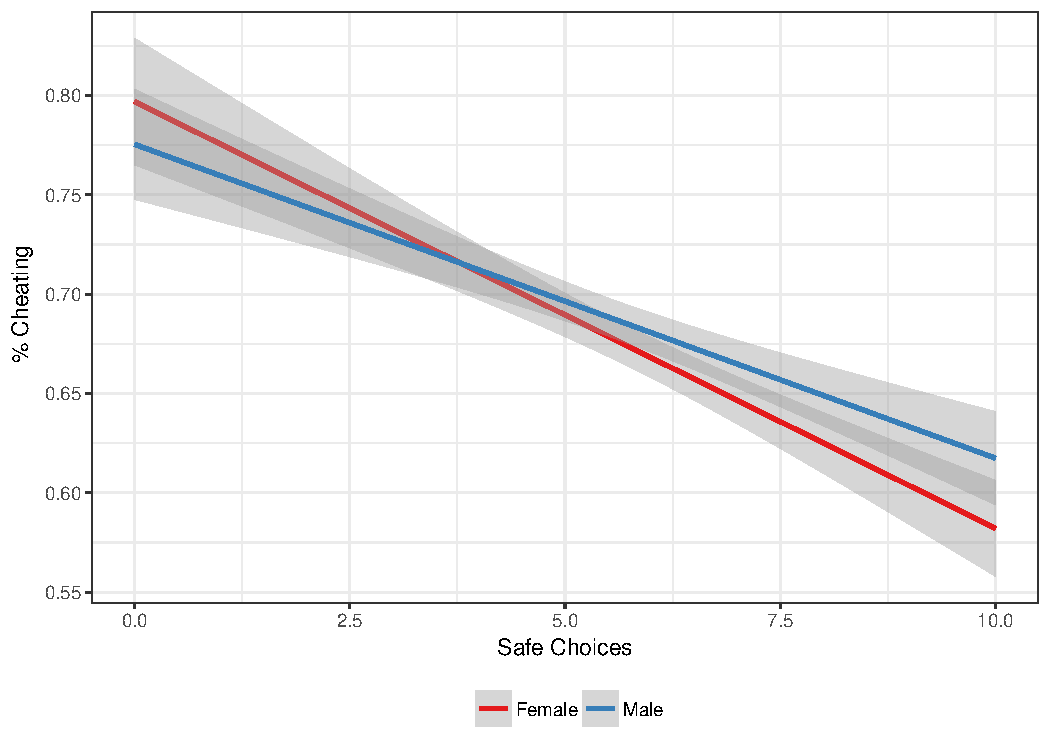
\includegraphics[width=.8\linewidth]{cheat_genderxsafechoices07Aug2017}
\caption{Gender by ability and audit rate}
\label{fig:frog}
\end{figure}


%\begin{SCfigure*}[\sidecaptionrelwidth][t]
\begin{figure}[tbhp]
\centering
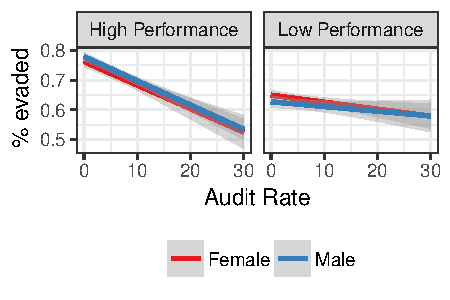
\includegraphics[width=.8\linewidth]{cheat_genderxability07Aug2017}
\caption{Cheating by ability type}\label{fig:side}
\end{figure}

%\end{SCfigure*}

\subsection*{Digital Figures}
\label{sec:figures}

%Only TIFF, EPS, and high-resolution PDF for Mac or PC are allowed for figures that will appear in the main text, and images must be final size. Authors may submit U3D or PRC files for 3D images; these must be accompanied by 2D representations in TIFF, EPS, or high-resolution PDF format.  Color images must be in RGB (red, green, blue) mode. Include the font files for any text. 

%Figures and Tables should be labelled and referenced in the standard way using the \verb|\label{}| and \verb|\ref{}| commands.

Figure \ref{fig:frog} shows an example of how to insert a column-wide figure. To insert a figure wider than one column, please use the \verb|\begin{figure*}...\end{figure*}| environment. Figures wider than one column should be sized to 11.4 cm or 17.8 cm wide. Use \verb|\begin{SCfigure*}...\end{SCfigure*}| for a wide figure with side captions.


\begin{table}%[tbhp]
\centering
\caption{Comparison of the fitted potential energy surfaces and ab initio benchmark electronic energy calculations}
\begin{tabular}{lrrr}
Species & CBS & CV & G3 \\
\midrule
1. Acetaldehyde & 0.0 & 0.0 & 0.0 \\
2. Vinyl alcohol & 9.1 & 9.6 & 13.5 \\
3. Hydroxyethylidene & 50.8 & 51.2 & 54.0\\
\bottomrule
\end{tabular}

\addtabletext{nomenclature for the TSs refers to the numbered species in the table.}
\end{table}


\matmethods{%Please describe your materials and methods here. This can be more than one paragraph, and may contain subsections and equations as required. Authors should include a statement in the methods section describing how readers will be able to access the data in the paper. 
%\subsection*{Subsection for Method}
%Example text for subsection.

The majority of participants were recruited from the University of Oxford in Oxford, the Universidad de Santiago (USACH) in Santiago and the Higher School of Economics (HSE) in Moscow. Oxford and HSE are elite universities, with a large proportion of students from families of high socio-economic status. Students at USACH, on the other hand, are very diverse with many from middle to low socio-economic backgrounds and first family members to attend university. Slightly over half of all subjects were males (51.5\% in UK, 52.2\% in Chile, and 52\% in Russia). The majority of subjects were in their late teens and 20s, with the median age being 22 years in UK and Chile, and 20 years in Russia. 

Subjects were paid the amount they kept/received in the Dictator Game, plus a randomly selected round from the first RET and decision module, plus one randomly selected round from the second RET and decision module, plus the results of the Risk Aversion Test and the Die treatment, when applied. ECU earnings were converted at the exchange rate of 300 ECUs per \pounds 1 in Oxford and 300 ECUs per 500 pesos in Santiago. The exchange rate in Moscow varied between 7 ECU and 9 ECU per Russian rouble to keep the total earnings relatively constant in USD dollars.\footnote{The exchange rate for Rouble was between 35 and 60 Roubles per USD, depending on when the session took place.}

All the data presented in this manuscript will be made available though the PNAS repository and Github. 
}

\showmatmethods{


} % Display the Materials and Methods section

\acknow{Please include your acknowledgments here, set in a single paragraph. Please do not include any acknowledgments in the Supporting Information, or anywhere else in the manuscript.}

\showacknow{} % Display the acknowledgments section

% \pnasbreak splits and balances the columns before the references.
% Uncomment \pnasbreak to view the references in the PNAS-style
% If you see unexpected formatting errors, try commenting out \pnasbreak
% as it can run into problems with floats and footnotes on the final page.
%\pnasbreak

% Bibliography
\bibliography{LibraryGender,dave}

\end{document}


Template information:



\dropcap{T}his PNAS journal template is provided to help you write your work in the correct journal format.  Instructions for use are provided below.

Note: please start your introduction without including the word ``Introduction'' as a section heading (except for math articles in the Physical Sciences section); this heading is implied in the first paragraphs. 

\section*{Guide to using this template on Overleaf}

Please note that whilst this template provides a preview of the typeset manuscript for submission, to help in this preparation, it will not necessarily be the final publication layout. For more detailed information please see the \href{http://www.pnas.org/site/authors/format.xhtml}{PNAS Information for Authors}.

If you have a question while using this template on Overleaf, please use the help menu (``?'') on the top bar to search for \href{https://www.overleaf.com/help}{help and tutorials}. You can also \href{https://www.overleaf.com/contact}{contact the Overleaf support team} at any time with specific questions about your manuscript or feedback on the template.

\subsection*{Author Affiliations}

Include department, institution, and complete address, with the ZIP/postal code, for each author. Use lower case letters to match authors with institutions, as shown in the example. Authors with an ORCID ID may supply this information at submission.

\subsection*{Submitting Manuscripts}

All authors must submit their articles at \href{http://www.pnascentral.org/cgi-bin/main.plex}{PNAScentral}. If you are using Overleaf to write your article, you can use the ``Submit to PNAS'' option in the top bar of the editor window. 

\subsection*{Format}

Many authors find it useful to organize their manuscripts with the following order of sections;  Title, Author Affiliation, Keywords, Abstract, Significance Statement, Results, Discussion, Materials and methods, Acknowledgments, and References. Other orders and headings are permitted.




\subsection*{Manuscript Length}

PNAS generally uses a two-column format averaging 67 characters, including spaces, per line. The maximum length of a Direct Submission research article is six pages and a PNAS PLUS research article is ten pages including all text, spaces, and the number of characters displaced by figures, tables, and equations.  When submitting tables, figures, and/or equations in addition to text, keep the text for your manuscript under 39,000 characters (including spaces) for Direct Submissions and 72,000 characters (including spaces) for PNAS PLUS.

\subsection*{References}

References should be cited in numerical order as they appear in text; this will be done automatically via bibtex, e.g. \cite{belkin2002using} and \cite{berard1994embedding,coifman2005geometric}. All references, including for the SI, should be included in the main manuscript file. References appearing in both sections should not be duplicated.  SI references included in tables should be included with the main reference section. 

\subsection*{Data Archival}

PNAS must be able to archive the data essential to a published article. Where such archiving is not possible, deposition of data in public databases, such as GenBank, ArrayExpress, Protein Data Bank, Unidata, and others outlined in the Information for Authors, is acceptable.

\subsection*{Language-Editing Services}
Prior to submission, authors who believe their manuscripts would benefit from professional editing are encouraged to use a language-editing service (see list at www.pnas.org/site/authors/language-editing.xhtml). PNAS does not take responsibility for or endorse these services, and their use has no bearing on acceptance of a manuscript for publication. 

\begin{figure}%[tbhp]
\centering
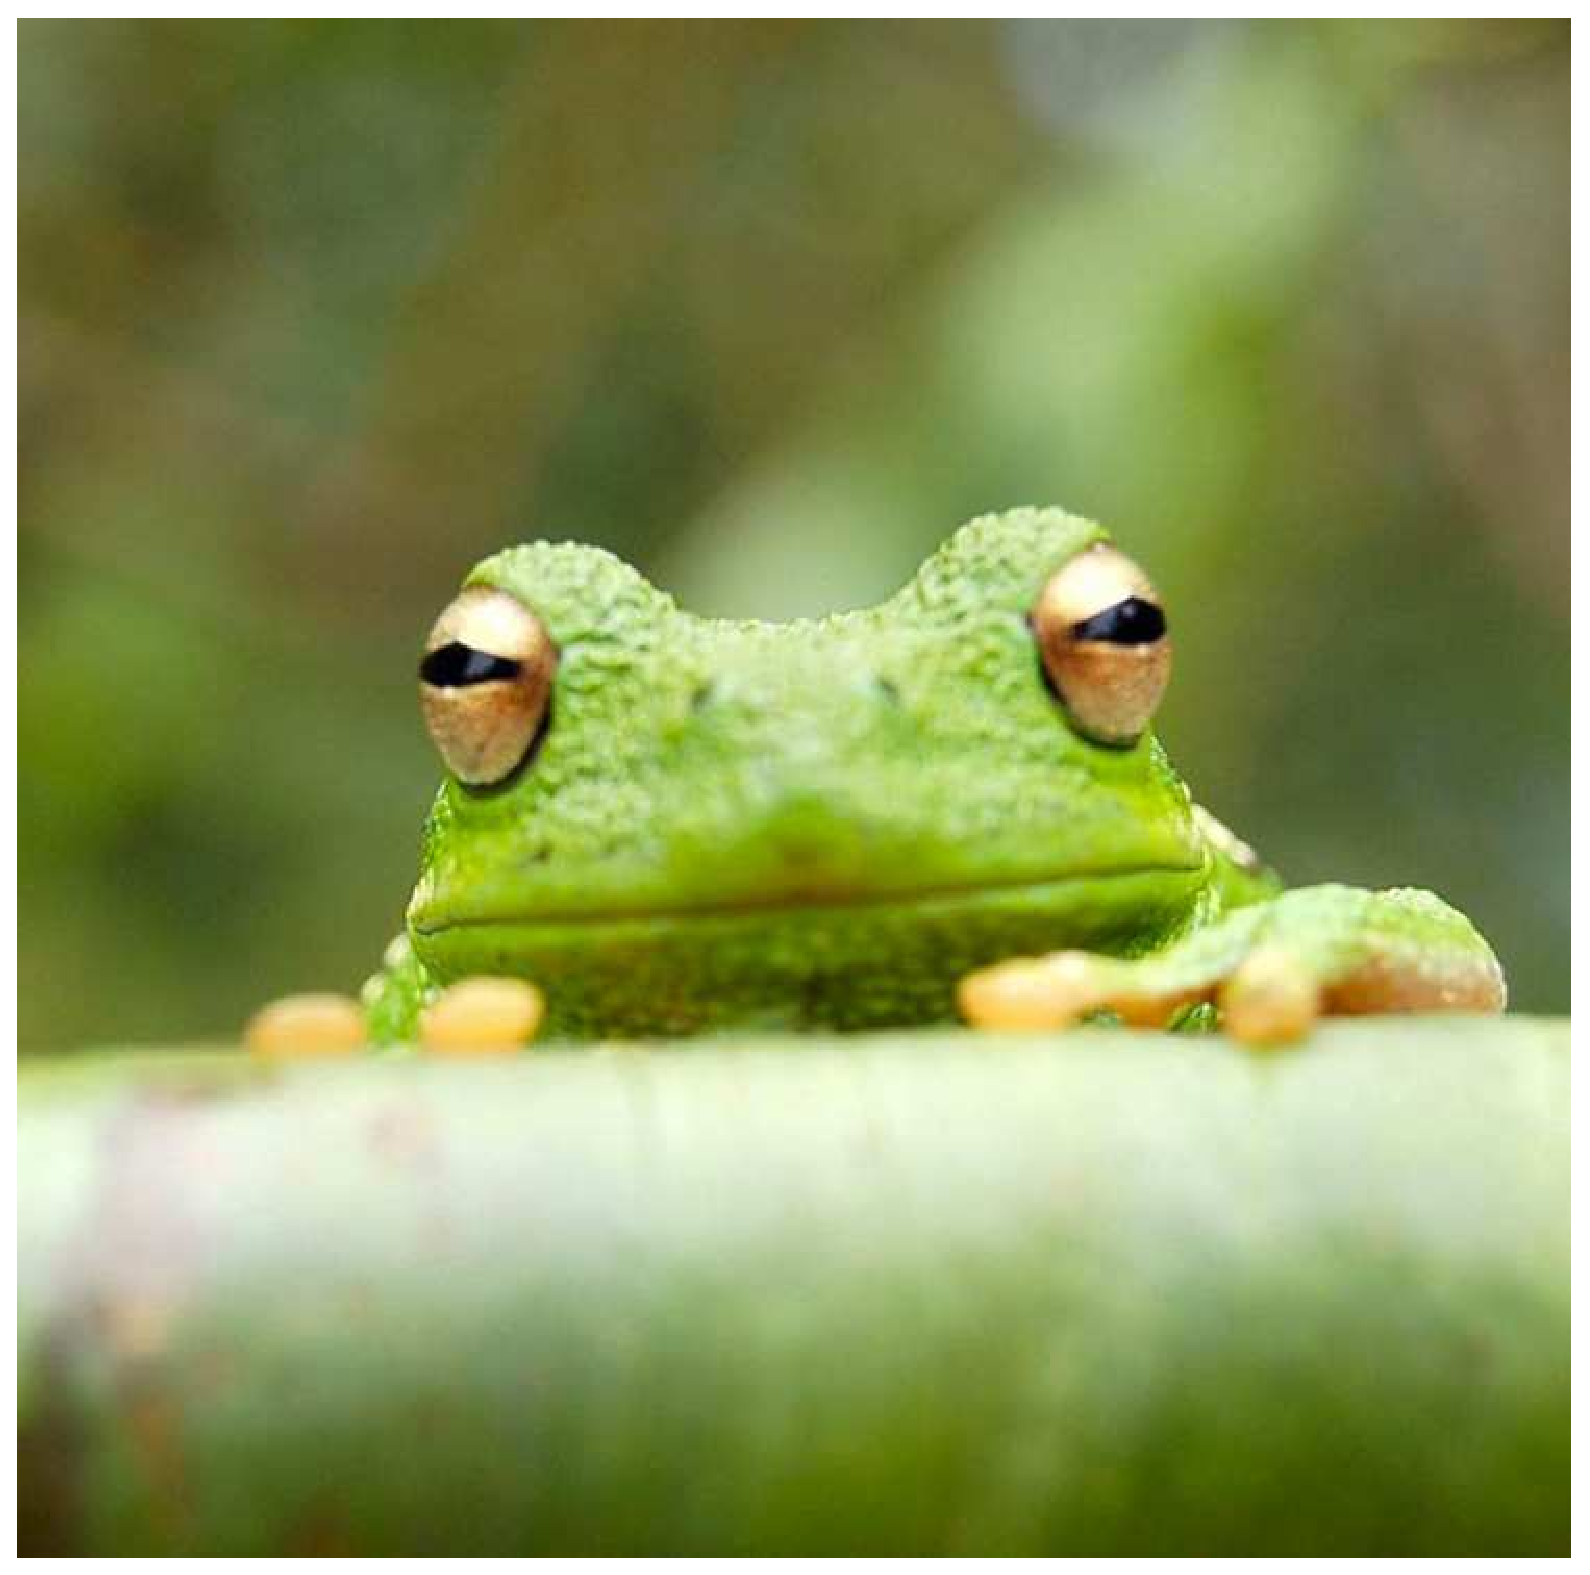
\includegraphics[width=.8\linewidth]{frog}
\caption{Placeholder image of a frog with a long example caption to show justification setting.}
\label{fig:frog}
\end{figure}


\begin{SCfigure*}[\sidecaptionrelwidth][t]
\centering
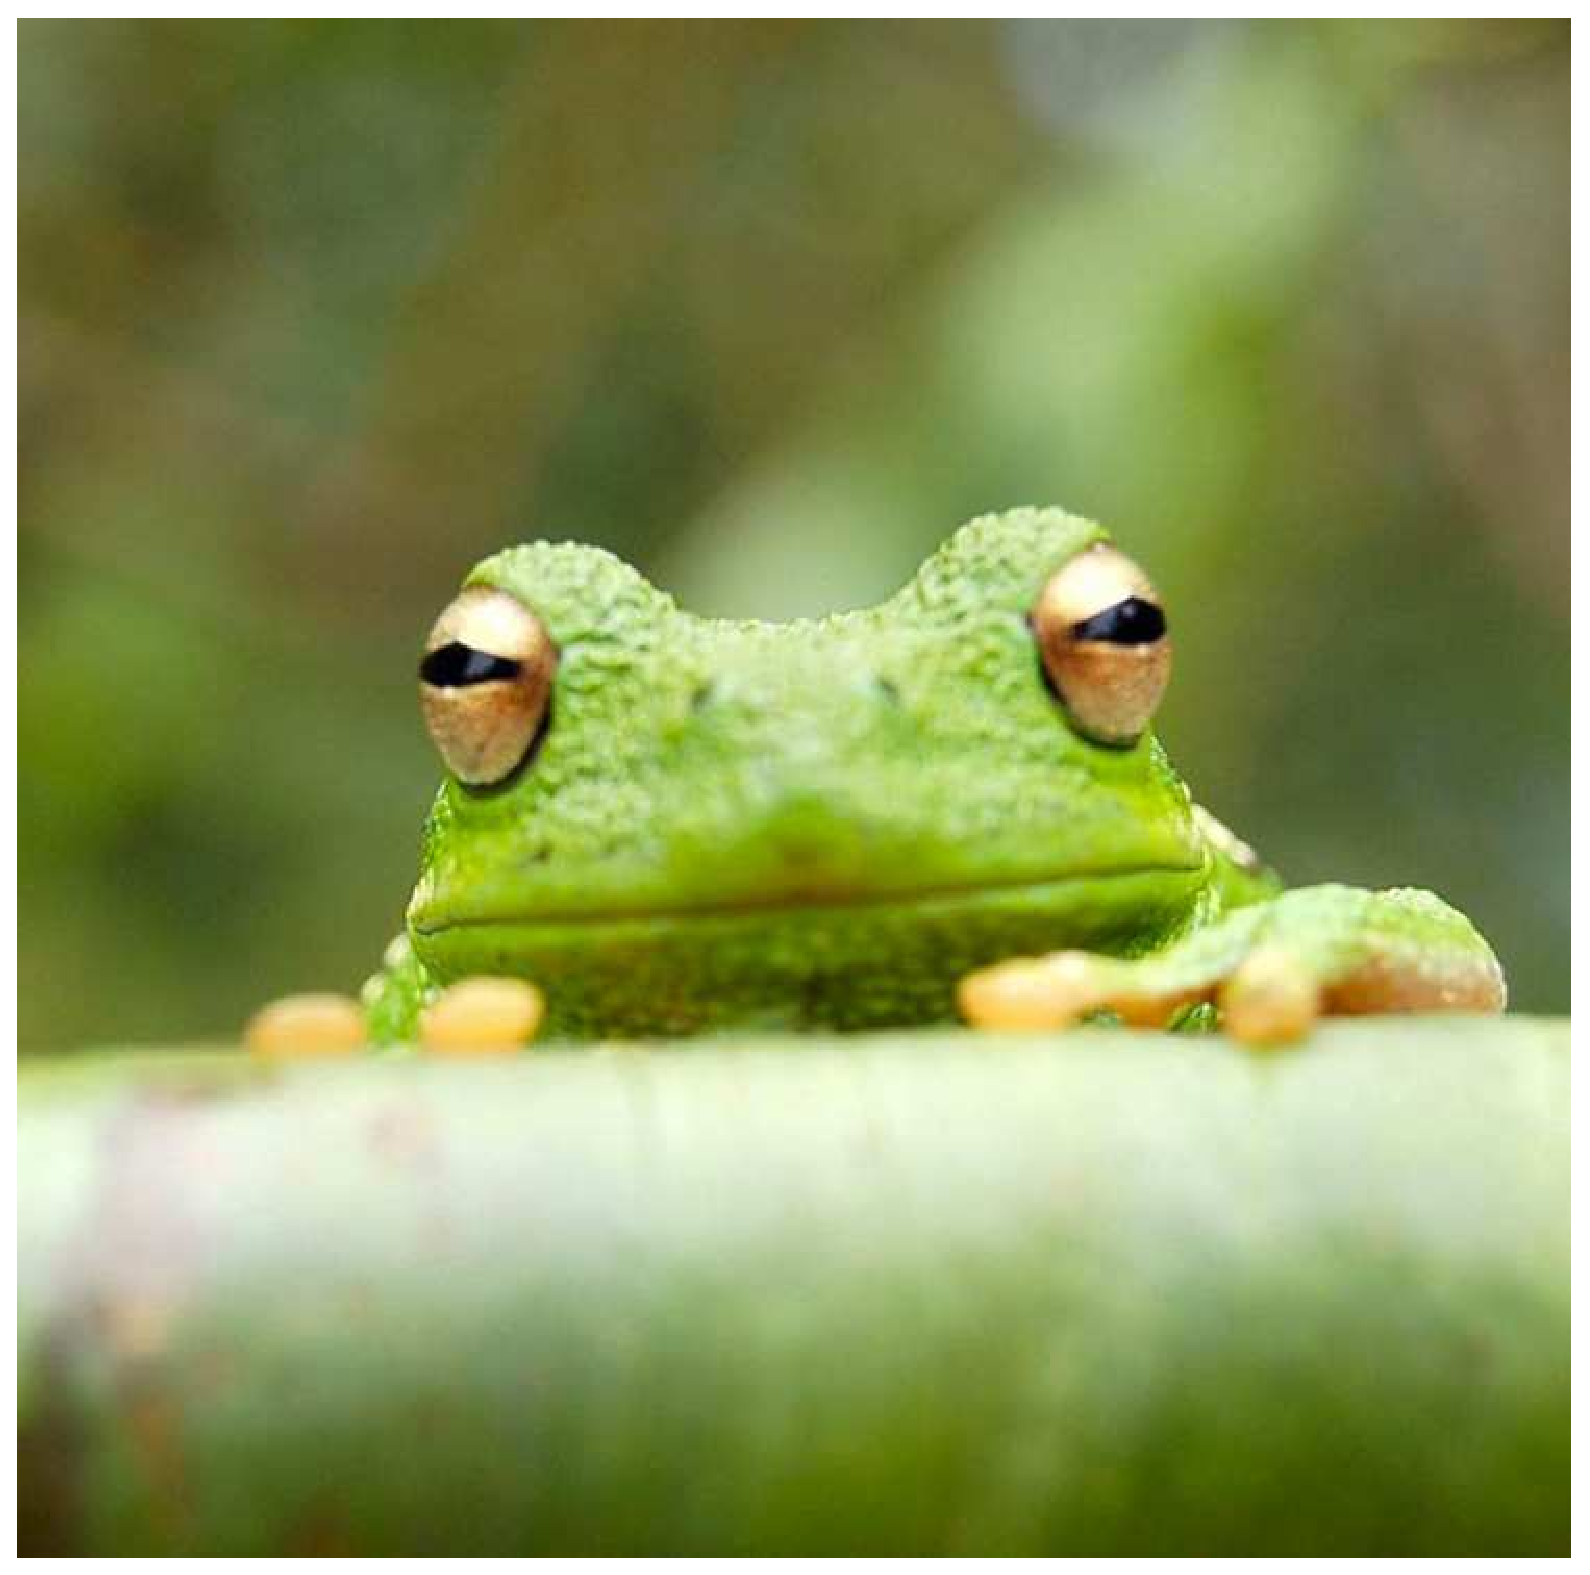
\includegraphics[width=11.4cm,height=11.4cm]{frog}
\caption{This caption would be placed at the side of the figure, rather than below it.}\label{fig:side}
\end{SCfigure*}

\subsection*{Digital Figures}
\label{sec:figures}

Only TIFF, EPS, and high-resolution PDF for Mac or PC are allowed for figures that will appear in the main text, and images must be final size. Authors may submit U3D or PRC files for 3D images; these must be accompanied by 2D representations in TIFF, EPS, or high-resolution PDF format.  Color images must be in RGB (red, green, blue) mode. Include the font files for any text. 

Figures and Tables should be labelled and referenced in the standard way using the \verb|\label{}| and \verb|\ref{}| commands.

Figure \ref{fig:frog} shows an example of how to insert a column-wide figure. To insert a figure wider than one column, please use the \verb|\begin{figure*}...\end{figure*}| environment. Figures wider than one column should be sized to 11.4 cm or 17.8 cm wide. Use \verb|\begin{SCfigure*}...\end{SCfigure*}| for a wide figure with side captions.

\subsection*{Single column equations}

Authors may use 1- or 2-column equations in their article, according to their preference.

To allow an equation to span both columns, options are to use the \verb|\begin{figure*}...\end{figure*}| environment mentioned above for figures, or to use the \verb|\begin{widetext}...\end{widetext}| environment as shown in equation \ref{eqn:example} below.

Please note that this option may run into problems with floats and footnotes, as mentioned in the \href{http://texdoc.net/pkg/cuted}{cuted package documentation}. In the case of problems with footnotes, it may be possible to correct the situation using commands \verb|\footnotemark| and \verb|\footnotetext|.

%% Do not use widetext if paper is in single column.
\begin{widetext}
\begin{align*}
(x+y)^3&=(x+y)(x+y)^2\\
       &=(x+y)(x^2+2xy+y^2) \numberthis \label{eqn:example} \\
       &=x^3+3x^2y+3xy^3+x^3. 
\end{align*}
\end{widetext}

\begin{table}%[tbhp]
\centering
\caption{Comparison of the fitted potential energy surfaces and ab initio benchmark electronic energy calculations}
\begin{tabular}{lrrr}
Species & CBS & CV & G3 \\
\midrule
1. Acetaldehyde & 0.0 & 0.0 & 0.0 \\
2. Vinyl alcohol & 9.1 & 9.6 & 13.5 \\
3. Hydroxyethylidene & 50.8 & 51.2 & 54.0\\
\bottomrule
\end{tabular}

\addtabletext{nomenclature for the TSs refers to the numbered species in the table.}
\end{table}

\subsection*{Supporting Information (SI)}

The main text of the paper must stand on its own without the SI. Refer to SI in the manuscript at an appropriate point in the text. Number supporting figures and tables starting with S1, S2, etc. Authors are limited to no more than 10 SI files, not including movie files. Authors who place detailed materials and methods in SI must provide sufficient detail in the main text methods to enable a reader to follow the logic of the procedures and results and also must reference the online methods. If a paper is fundamentally a study of a new method or technique, then the methods must be described completely in the main text. Because PNAS edits SI and composes it into a single PDF, authors must provide the following file formats only.

\subsubsection*{SI Text}

Supply Word, RTF, or LaTeX files (LaTeX files must be accompanied by a PDF with the same file name for visual reference).

\subsubsection*{SI Figures}

Provide a brief legend for each supporting figure after the supporting text. Provide figure images in TIFF, EPS, high-resolution PDF, JPEG, or GIF format; figures may not be embedded in manuscript text. When saving TIFF files, use only LZW compression; do not use JPEG compression. Do not save figure numbers, legends, or author names as part of the image. Composite figures must be pre-assembled.

\subsubsection*{3D Figures}

Supply a composable U3D or PRC file so that it may be edited and composed. Authors may submit a PDF file but please note it will be published in raw format and will not be edited or composed.

\subsubsection*{SI Tables}

Supply Word, RTF, or LaTeX files (LaTeX files must be accompanied by a PDF with the same file name for visual reference); include only one table per file. Do not use tabs or spaces to separate columns in Word tables.

\subsubsection*{SI Datasets} 

Supply Excel (.xls), RTF, or PDF files. This file type will be published in raw format and will not be edited or composed. 

\subsubsection*{SI Movies}

Supply Audio Video Interleave (avi), Quicktime (mov), Windows Media (wmv), animated GIF (gif), or MPEG files and submit a brief legend for each movie in a Word or RTF file. All movies should be submitted at the desired reproduction size and length. Movies should be no more than 10 MB in size. 

\subsubsection*{Still images}

Authors must provide a still image from each video file. Supply TIFF, EPS, high-resolution PDF, JPEG, or GIF files. 

\subsubsection*{Appendices}

PNAS prefers that authors submit individual source files to ensure readability. If this is not possible, supply a single PDF file that contains all of the SI associated with the paper. This file type will be published in raw format and will not be edited or composed.

\matmethods{Please describe your materials and methods here. This can be more than one paragraph, and may contain subsections and equations as required. Authors should include a statement in the methods section describing how readers will be able to access the data in the paper. 

\subsection*{Subsection for Method}
Example text for subsection.
}

\showmatmethods{


} % Display the Materials and Methods section

\acknow{Please include your acknowledgments here, set in a single paragraph. Please do not include any acknowledgments in the Supporting Information, or anywhere else in the manuscript.}

\showacknow{} % Display the acknowledgments section

% \pnasbreak splits and balances the columns before the references.
% Uncomment \pnasbreak to view the references in the PNAS-style
% If you see unexpected formatting errors, try commenting out \pnasbreak
% as it can run into problems with floats and footnotes on the final page.
%\pnasbreak

% Bibliography
